\chapter{Desarrollo del trabajo}


\section{Algoritmo de Shor para buscar k-ciclos}

Como ya sabemos, el algoritmo de Shor nos permitiría una eficiencia mayor a la hora de calcular el periodo de la función $2^x \equiv 1 \pmod N$, lo que nos permitiría realizar la búsqueda de ciclos de una mayor longitud.



\subsection{Breve introducción del algoritmo de Shor}
(buscar referencias y hacer una introducción al algoritmo de Shor)



\subsection{Idea general}

Como podemos ver en la fórmula de los k-ciclos \ref{FormulakCicloCollatzAlterna}, para un k-ciclo obtenemos $k$ fracciones con denominador $N=2^L-3^X$ y cuyos numeradores son $2^{y_i} - 1$ multiplicados por un respectivo factor que podemos llamar $F_i = 3^{X - X_i} 2^{L_{i-1}} 2^{x_i}$.
$\\$


De esta manera, después de calcular nuestro $r$ de forma que $2^r \equiv 1 \pmod N$, si pudiéramos encontrar los $k$ términos $y_i$ de forma que fueran múltiplos de $r$, entonces habríamos encontrado automáticamente un k-ciclo y por tanto un contraejemplo de la conjetura, demostrando su falsedad.
$\\$


De todas formas, no debemos olvidar que el hecho de no encontrar k-ciclos no probaría nada, ni siquiera la inexistencia de estos k-ciclos, pues podría existir un k-ciclo cuyo denominador $N$ no dividiera a alguno de sus numeradores (o a ninguno), y sin embargo si dividir al producto $\sum\limits_{i=1}^k F_i (2^{y_i} - 1)$. 
$\\$

Lo que haremos pues, será iterar sobre la longitud del k-ciclo $L$, Utilizaremos que $Y \approx \frac{L}{1+log_2(3)}$ y que $X \approx log_2(3) Y$ para obtener $X$ e $Y$ redondeando la expresión al número entero más cercano.
$\\$


En cada iteración de $L$, buscaremos el periodo $r$ (que podremos buscar de forma más eficiente si utilizamos la parte cuántica del algoritmo de Shor), y comprobaremos si $r$ divide a $Y$, puesto que nos interesa buscar $y_1$, $y_2$, ... múltiplos de $r$ (y recordemos que $Y=y_1+y_2+...+y_k$)
$\\$


Utilizaremos también algunas restricciones para optimizar el proceso.



\subsection{Restricción de la longitud de los ciclos}
Sabemos gracias a (\cite{LowerBoundsCycleLength}) que la longitud de un ciclo cualquiera debe ser de la forma:

$$L = 301994a + 17087915b + 85137581c$$

con $a,b,c \in \mathbb N$  y  $ac=0$
$\\$


Dicho de otra forma, la longitud de un ciclo sólo puede ser de dos formas:
$$L = 301994a + 17087915b$$
$$L = 17087915b + 85137581c$$

Por tanto, en lugar de iterar directamente sobre $L$ ($L=1, L=2,...$), podemos iterar simultáneamente en un bucle doble sobre $b=1,2,...$ y sobre $a=0,1,...$ y $c=0,1,...$ cubriendo así todos los $L$ posibles.
$\\$

Por ejemplo si $a=1$, $b=1$, obtendríamos $L=17.389.909$.

Después calcularíamos $Y = L \frac{1}{1+log_2 3}$

Luego $X = log_2 3 Y = L \frac{log_2 3}{1+log_2 3}$
$\\$


Esto desde luego nos permitiría optimizar mucho nuestro código, ya que estamos descartando muchas longitudes de ciclos que sabemos que no pueden existir debido a (\cite{LowerBoundsCycleLength}).


\subsection{Restricción sobre la dimensión $k$ de un k-ciclo}
Utilizaremos también el hecho de que no existen k-ciclos con $k \leq 91$ (\cite{hercher2023collatzmcycles}).

Esto significa que habrán al menos $92$ variables $y_i$ que necesitarán ser múltiplo de $r$.

como todas las $y_i$ deben ser múltiplos de $r$, entonces $Y=\sum\limits_{i=0}^s y_i$ deberá ser también múltiplo de $r$, por tanto eso nos restringe los posibles valores de $Y$.
$\\$


Lo que ocurrirá normalmente, y que nos impedirá encontrar k-ciclos, será que $r$ no dividirá a $Y$, de hecho será probablemente mayor.
$\\$


Encontrar un $r$ que divida a nuestro $Y$ es pues el primer paso, que nos permitirá descartar la mayoría de iteraciones sin necesidad de proseguir con el algoritmo.

En caso de que encontráramos un $r$ que sí dividiera a nuestro $Y$, tendríamos que proseguir, verificando que divida a cada uno de los $y_i$, ya que por ejemplo en un 2-ciclo podríamos obtener $r=4$, $Y=8$ pero $y_1 = 3$ y $y_2 = 5$ (aunque sepamos $k=2$ no es un ciclo posible, se entiende el ejemplo).







\subsection{Algoritmo clásico para la búsqueda del periodo}
Un algoritmo clásico en python para el cálculo del periodo podría ser el siguiente:

\begin{verbatim}
#Esta funcion busca el menor r>0 que verifica 2^r=1 (mod N) y que sea menor que Y
#Devolvera 0 si no existe y r>0 si existe
def CalculoPeriodoClasico(N, Y, debug = False):
    r=0
    mod = 1; #Comenzamos para almacenar la congruencia módulo de los respectivos 2^i
    if debug:
        print ("N:", N)
        print ("Y:", Y)
        
    #Si N es multiplo de 2 no tiene sentido seguir,
    #nunca encontraremos r>0 tal que 2^r=1(mod N)
    if (N%2 == 0):
        return 0
    
    for i in range(1, Y):
        #Multiplicamos por 2 para obtener el siguiente 2^i
        mod = mod*2
        if mod>N:
            #Como estamos multiplicando por 2, como maximo solo supera,
            #a N una vez, es decir mod<2N
            #Por lo tanto esto es análogo a hacer mod%N pero más rapido
            mod = mod - N
        if debug:
            print (i, ": ", mod)
        if mod == 1:
            #Cuando obtenemos 2^i = 1 mod N devolvemos el indice i
            return sp.Integer(i)
    
    #Si hemos acabado el for y no ha encontrado r devolvemos 0
    return 0
\end{verbatim}

En este algoritmo (seguro que se puede optimizar), nos detenemos si llegamos a $Y$, puesto que si $r>Y$ entonces nunca será múltiplo, de hecho podríamos optimizar el algoritmo comprobando simplemente los divisores de $Y$ por ejemplo.

Incluso podríamos utilizar también la restricción de que $s\geq92$ para iterar únicamente sobre los divisores de $Y$ menores de $\frac{Y}{92}$, ya que se deberá verificar que al menos $92$ valores de $y_i$ deberán ser múltiplos de $r$.

Aunque realmente con la restricción de $\sqrt{Y}$ (el mayor divisor distinto de $Y$) estaríamos restringiendo más que con $\frac{Y}{92}$ en prácticamente todos los casos de interés, puesto que trabajaremos con valores de $Y$ grandes (mucho mas que $92^2$)



\subsection{Algoritmo cuántico para la búsqueda del periodo}
Introducir aquí la implementación de la parte cuántica de Shor



\subsection{Algoritmo de búsqueda de k-ciclos}
Definimos primero una función que calcule el periodo de forma cuántica o clásica en función de una variable booleana:

\begin{verbatim}
def CalculoPeriodo(N, Y, esCuantico = False, debugPeriodo = False):
    if esCuantico:
        return CalculoPeriodoCuantico(N, Y, debugPeriodo)
    else:
        return CalculoPeriodoClasico(N, Y, debugPeriodo)
\end{verbatim}
$\\$


Ahora definimos una función para buscar los ciclos de una determinada longitud L:

\begin{verbatim}
#Esta funcion busca k-ciclos de longitud L
def BuscarCiclo(L, debug = False, debugPeriodo = False):
    #Establecemos este numero grande para debuggear N grande
    sys.set_int_max_str_digits(10000000)
    
    #Guardamos la constante log2(3) (la usaremos constantemente)
    log23 = np.log2(3)
    #Guardamos esta constante mediante la cual calculamos Y: (Y = Kly * L)
    Kly = 1/(1+log23) 
    
    #Mostramos L:
    if debug:
        print("L: ", L)
        
    #Calculamos Y en función de nuestro L
    Y = round(Kly * L) 
    #Mostramos Y:
    if debug:
        print("Y: ", Y)
        
    #Calculamos X en función de Y (que a su vez esta en función de L)
    X = round(log23 * Y)
    #Mostramos X:
    if debug:
        print("X: ", X)
        
    #Calculamos N = 2^L - 3^X
    N = pow(2,L) - pow(3,X)
    #Mostramos N:
    if debug:
        print("N: ", N)

    
    #Calculamos el periodo de con la función CalculoPeriodo
    r = CalculoPeriodo(N, Y, False, debugPeriodo) 
    
    #Mostramos el periodo obtenido (r=0 significa periodo no valido,
    #bien porque N es multiplo de 2 o porque se ha superado el limite (Y)
    if debug:
        print("r:", r)
        
    #Comprobamos que r divida a Y (y no sea 0)
    if r!=0:
        print ("r>0!")
        if Y%r == 0:
            if BusquedaYi(r, Y):
                print ("¡¡¡¡¡CICLO ENCONTRADO!!!!!")
                
    return(r)
\end{verbatim}
$\\$


La función BusquedaYi(r, Y) se encargaría de buscar una combinación válida de $y_i$ que sean múltiplos de $r$ y cuya suma sea $Y$.
$\\$

Por último buscamos todos los ciclos que verifiquen la condición $$L = 301994a + 17087915b$$ o bien $$L = 17087915b + 85137581c$$
\begin{verbatim}
#Buscamos primero el ciclo en que a=0, c=0:
BuscarCiclo(17087915, True, False)

for i in range(1, 1001):  #Iteramos la variable a entre 1 y 1000 incluidos
    for j in range (1, 1001):  #Iteramos la variable b entre 1 y 1000 incluidos
        #Buscamos k-ciclos con longitud L teniendo c=0
        L = 301994 * i + 17087915 * j  
        BuscarCiclo(L, True, False)
        #Buscamos k-ciclos con longitud L teniendo a=0
        L = 85137581 * i + 17087915 * j 
        BuscarCiclo(L, True, False)
\end{verbatim}




\section{Algoritmo Cuántico usando la representación binaria}

Utilizando la representación binaria de un número $n \in \mathbf{N}$, podemos realizar una aplicación de la función de Collatz $T$ (\ref{T(n)}), de la siguiente manera:

Si el último dígito del número binario es $0$, entonces lo eliminamos ya que el número es par y quitarlo equivale a dividir entre $2$.

Si por el contrario el último dígito es $1$ eso significa que el número es impar y lo que hacemos es añadirle un $1$ al final (obteniendo $2n+1$) y sumarlo al número original (obteniendo $3n+1$).
Sabemos por supuesto que ese número será par y acabará en $0$, por tanto por último eliminaremos el último dígito para así obtener finalmente $\frac{3n+1}{2}$.
$\\$

Veámoslo con un ejemplo pequeño:

Si $n=11$, tenemos la sucesión $\{11, 17, 26, 13, 20, 10, 5, 8, 4, 2, 1,...\}$ que evidentemente alcanza el número $1$.

Escribimos $n$ en binario: $1011$.

Ahora como es impar, sumaríamos $1011$ y $10111$ y eliminaríamos el último $0$ obteniendo: $10001$ (que es nuestro $17$).

De nuevo es impar así que sumamos $10001$ y $100011$ y eliminamos el último $0$ obteniendo $11010$ ($26$).

Ahora es par, así que eliminamos un $0$ adicional obteniendo $1101$ ($13$).

De nuevo impar, sumamos $1101$ y $11011$ eliminando el último $0$ y obtenemos ahora: $10100$ ($20$).

Ahora $10100$ no solamente es par, si no que además es divisible entre $4$ (tiene dos $0$ al final), así que podemos quitarlos directamente (esto equivaldría a realizar el paso de quitar el último $0$ dos veces).

Obtenemos $101$ ($5$) por tanto sumamos $101$ y $1011$ obteniendo $1000$ ($8$).

Y ya llegaríamos finalmente a $1$ después de eliminar los $3$ últimos ceros.


\subsection{Idea general del algoritmo cuántico}
Utilizando un conjunto de puertas NOT, CNOT, CCNOT, ... podemos construir un sumador cuántico (de forma similar al sumador clásico utilizando compuertas XOR etc).
$\\$

Esto en principio no sería muy relevante de por sí, ya que será más eficiente hacerlo de forma clásica, pero podemos colocar primero el estado en superposición con puertas Hadamard, para luego aplicar el sumador.
$\\$

De esta forma trataremos de evaluar $p$ iteraciones de Collatz para los $2^q$ simultáneamente, probando a la vez que la conjetura es cierta para todos los $n\leq2^q$ que tengan un Tiempo de Parada menor a $p$.
$\\$

Necesitaremos sin embargo muchos qubits si queremos lograr números elevados, ya que necesitaremos $q$ qubits para cubrir y un qubit extra por cada iteración que realicemos (ya que al ser una superposición no podremos comprobar si el último dígito es $0$ o $1$).
$\\$

Sin embargo, podemos ver que el tiempo de parada crece excepcionalmente lento (buscar referencias de relación de tiempo de parada).
$\\$

La siguiente tabla muestra los mayores tiempos de parada para los números menores que cierta potencia de $10$:

\begin{table}[]
    \centering
    \begin{tabular}{|c|c|}
    \hline
        Valor Máximo & Tiempo de Parada \\
    \hline
        $10$ & $19$ \\
        $100$ & $118$ \\
        $1000$ & $178$ \\
        $10^5$ & $261$ \\
        $10^6$ & $350$ \\
        $10^7$ & $524$ \\
        $10^8$ & $685$ \\
        $10^9$ & $949$ \\
        $10^{10}$ & $986$ \\
        $10^{11}$ & $1132$ \\
        $10^{12}$ & $1348$ \\
    \hline
    \end{tabular}
    \caption{Tiempo de Parada máximo}
    \label{tab:maximum stopping time}
\end{table}


Por tanto, es posible que con algunos pocos miles de qubits ya seamos capaces de hallar resultados interesantes.



\subsection{Pasos del algoritmo cuántico}
El primer paso es colocar los primeros $m$ qubits en un estado de superposición aplicándole una puerta Hadamard a cada qubit. De esta forma tendremos un número binario en superposición, si midiéramos los $m$ primeros qubits obtendríamos con igual probabilidad un número binario de $m$ dígitos (un número comprendido entre $0$ y $2^m-1$).
$\\$

A continuación nos generaremos una función que aplicaremos en cada uno de los pasos correspondientes al tiempo de parada. Dicha función aceptará como argumentos de entrada $3$ qubits ($2$ dígitos del número binario y un tercer qubit que contendrá el acarreo). Como salida, devolverá un qubit con un dígito con el resultado y otro para el acarreo. Dichas salidas las añadiremos como inputs de entrada para la siguiente iteración, que junto con el siguiente dígito formarán los 3 inputs de entrada de la función. (añadir diagrama para facilitar la comprensión).
$\\$

Veámoslo más claro con un ejemplo:

Supongamos que queremos computar $4$ dígitos binarios en un tiempo de parada máximo de $6$:

Tendríamos los $4$ primeros qubits ($q_0$, $q_1$, $q_2$ y $q_3$) reservados para los $4$ dígitos.

Aplicaríamos nuestra función primero con entradas $0$, $q_0$, $q_1$ (Comenzamos con acarreo $0$).

Dicha función nos devolvería un output $r_1$, $a_1$.

A continuación aplicaríamos de nuevo nuestra función con las entradas $r_1$, $a_1$, $q_1$.
$\\$

Como podemos ver, el qubit $q_0$ ya no ha sido necesario en esta iteración (ni será necesario en un futuro) y tampoco lo será el qubit que representa el acumulador inicial $a_0=|0\rangle$ por lo tanto podemos ir reciclando estos qubits (o no hacerlo pero se necesitarían qubits auxiliares adicionales).
$\\$

Deberemos tener en cuenta que cada vez que vez que apliquemos la función (aplicación de $\frac{3n+1}{2}$), dejaremos un qubit ($r_i$), que no podremos analizar sin colapsarlo.
$\\$

Cuando acabemos de aplicar la función $p$ veces, habremos obtenido un $p+m+1$ qubits (comprobar), pero suponiendo que los números menores que $2^m$ tengan un tiempo de parada inferior a $p$, deberíamos haber obtenido a pesar de la superposición un valor de $|1\rangle$ en el primer o segundo qubit y un valor de $|0>$ en el resto (ya que  nos encontraríamos ya en el ciclo $\{ 1, 2 \}$).
$\\$

Quedaría por último comprobar que esto es cierto aplicando diversas estrategias para verificar que la medición ha resultado así por que efectivamente nos encontramos en el estado $|100\cdots0\rangle$ o en el $|0100\cdots0\rangle$, y no porque nos encontremos en una superposición y por azar cuántico nos haya dado la medición $100\cdots0$ o $0100\cdots0$ (comprobar como funcionaría esto).


\subsection{Ejemplo de algoritmo cuántico}
Supongamos que queremos comprobar computacionalmente hasta $n<2^4$, necesitaremos por tanto $4$ qubits para la representación binaria.

Tenemos pues $n = 2^3n_3 + 2^2n_2 + 2n_1 + n_0$ con $n\in\{0,1,\cdots,15\}$ y $n_3,n_2,n_1,n_0\in{0,1}$, y lo representaremos por el estado $|q_3q_2q_1q_0\rangle$.

Por ejemplo el estado $|q_3q_2q_1q_0\rangle = |1011\rangle$ corresponderá a $n=2^3 + 2 + 1 = 11$.

Ahora queremos implementar la suma de $n=2^3n_3 + 2^2n_2 + 2n_1 + n_0$ con $2n+1=2^4n_3 + 2^3n_2 + 2^2n_1 + 2n_0 + 1$

(revisar tabla, no está del todo bien)
\begin{center}
     \begin{tabular}{|c|c|c|c|c|c|}
        \hline
         & & $q_3$ & $q_2$ & $q_1$ & $q_0$ \\
         & $q_3$ & $q_2$ & $q_1$ & $q_0$ & 1 \\
        \hline
        $|(q_3\cdot q_2) \rangle$ & 
        $|q_3 \oplus (q_3\cdot q_2) \rangle$ & 
        $|(q_3 \oplus q_2) \oplus (q_2\cdot q_1) \rangle$ & 
        $|(q_2 \oplus q_1) \oplus (q_1\cdot q_0) \rangle$ & $|(q_1 \oplus q_0) \oplus (q_0\cdot1) \rangle$ & $|q_0\oplus1\rangle$ \\
        \hline
    \end{tabular}
\end{center}

Para ello realizaremos como hemos comentado una función que sume dos qubits (dígitos) teniendo en cuenta el acarreo anterior y devuelva un dígito resultado y un acarreo.
Veamos una tabla de verdad:

\begin{center}
    \begin{tabular}{|c|c|c||c|c|c|}
        \hline
        $a_0$ & $q_0$ & $q_1$ & $a_1$ & $r_1$\\
        \hline
        \hline
        0 & 0 & 0 & 0 & 0 \\
        0 & 0 & 1 & 0 & 1 \\
        0 & 1 & 0 & 0 & 1 \\
        0 & 1 & 1 & 1 & 0 \\
        \hline
        1 & 0 & 0 & 0 & 1 \\
        1 & 0 & 1 & 1 & 0 \\
        1 & 1 & 0 & 1 & 0 \\
        1 & 1 & 1 & 1 & 1 \\
        \hline
    \end{tabular}
\end{center}

Vemos que la primera mitad de la tabla de verdad (correspondiente a $a_0=0$), es simplemente una suma sin acarreo entre $q_0$ y $q_1$. Es decir una puerta XOR clásica entre $q_0$ y $q_1$ para hallar $r_1$ y una puerta AND para el acarreo $a_1$. 

La puerta XOR equivaldría en cuántica a dos puertas CNOT, de $q_0$ a $r_1$ y de $q_1$ a $r_1$:

(insertar imagen de las 2 puertas CNOT)

\begin{figure}
    \centering
    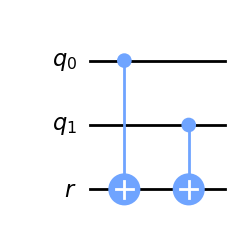
\includegraphics[width=0.5\linewidth]{XOR Cuantica.png}
    \caption{XOR Cuántica}
    \label{fig:XORCuantica}
\end{figure}

La puerta AND equivaldría cuánticamente a una puerta de Toffoli (CCNOT) con $q_0$ y $q_1$ como control y $r_1$ como objetivo.

(insertar imagen de la CCNOT)


Para la segunda mitad de la tabla ($a_0=1$) tendremos que para obtener $r_1$ basta con invertir el resultado de la tabla superior, es decir aplicar una puerta NOT, por tanto a la doble puerta CNOT de la tabla anterior le añadiremos una CNOT con $a_0$ como control para obtener el valor de $r_1$ en general.

(insertar imagen de las 3 puertas CNOT)


Para el valor de $a_1$, tendremos que es $0$ únicamente cuando $q_0$ y $q_1$ son $0$ simultáneamente, por tanto equivaldría a una CCNOT, pero con los qubits de control invertidos (que se puede lograr invirtiendo $q0$ y $q_1$ aplicando una CCNOT y volviéndolos a invertir para quedar como al inicio).

(insertar imagen de las 3 puertas CCNOT)

Una forma más sencilla de ver la salida de $a_1$ es observar que valdrá $1$ cuando $2$ o $3$ de los qubits $a_0$, $q_0$ y $q_1$ valgan $1$, y valdrá $0$ en caso contrario, cuando sólamente 1 de ellos o ninguno tenga valor $0$.
Esto lo podemos representar cuánticamente como 3 puertas CCNOT con qubits de control $a_0$ y $q_0$, $a_0$ y $q_1$, $q_0$ y $q_1$ respectivamente:

(insertar imagen de las 3 puertas CCNOT)

Esto es debido a que si únicamente 2 de los 3 qubits tienen valor $1$, se activará únicamente la puerta CCNOT que los tenga como qubits de control, mientras que si están los $3$ activados, se activarán las 3 puertas CCNOT (dando como resultado $1$ en el qubit $r1$).

El circuito final de nuestra función cuántica nos quedaría de la siguiente manera:

(insertar imagen del circuito de la función suma)

$\\$

Ahora la idea es como comentábamos más arriba aplicar dicha función de forma recursiva como mostraremos en el siguiente cuadro:

\begin{center}
    \begin{tabular}{c|c|c|c|c}
        $a_0=0$ & $r_1$ &  \\
        $q_0$   & $a_1$ & $r_2$ \\
        $q_1$   & $q_1$ & $a_2$ \\
                & $q_2$ & $q_2$
    \end{tabular}
\end{center}


$f(0,q_0,q_1) = (r_1, a_1)$
$f(a_1,q_1,q_2) = (r_2, a_2)$
$f(a_2,q_2,q_3) = (r_3, a_3)$
.
.
.
$f(a_$


\section{Problemas QUBO}
(Analizar si se puede formular algo como un problema de optimización, por ejemplo minimizar la distancia entre $\frac{X}{Y}-log_2 3$ o algo similar).
